\documentclass[10pt]{beamer}
\usetheme[
%%% option passed to the outer theme
%    progressstyle=fixedCircCnt,   % fixedCircCnt, movingCircCnt (moving is deault)
  ]{Feather}

% If you want to change the colors of the various elements in the theme, edit and uncomment the following lines

% Change the bar colors:
%\setbeamercolor{Feather}{fg=red!20,bg=red}

% Change the color of the structural elements:
%\setbeamercolor{structure}{fg=red}

% Change the frame title text color:
%\setbeamercolor{frametitle}{fg=blue}

% Change the normal text color background:
%\setbeamercolor{normal text}{fg=black,bg=gray!10}

%-------------------------------------------------------
% INCLUDE PACKAGES
%-------------------------------------------------------

% General
\usepackage[utf8]{inputenc}
\usepackage[portuguese]{babel}
\usepackage[T1]{fontenc}
\usepackage{helvet}

% Code syntax highlight
\usepackage{setspace}
\usepackage{color}
\usepackage{listings}

% Specify table cell length
\usepackage{array}

% Hyperlink reference
\usepackage{hyperref}

%-------------------------------------------------------
% DEFFINING AND REDEFINING COMMANDS
%-------------------------------------------------------

% colored hyperlinks
\newcommand{\chref}[2]{
  \href{#1}{{\usebeamercolor[bg]{Feather}#2}}
}

%-------------------------------------------------------
% Configure syntax highlight
%-------------------------------------------------------
\lstset{
  backgroundcolor=\color{white},
  breaklines=true,
  commentstyle=\color{green},
  extendedchars=true,
  frame=single,
  keepspaces=true,
  keywordstyle=\color{blue},
  language=Ruby,
  numbers=left,
  numbersep=10pt,
  numberstyle=\small\color{gray},
  rulecolor=\color{black},
  stringstyle=\color{blue},
  tabsize=2
}
%-------------------------------------------------------
% INFORMATION IN THE TITLE PAGE
%-------------------------------------------------------

% [] is optional - is placed on the bottom of the sidebar on every slide
% is placed on the title page
\title[] { 
\textbf{Kuniri Project}
}

\subtitle[An overview] {
}

\author[kuniri presentation] {
Rodrigo Siqueira Jordão
}

\date{\today}

%-------------------------------------------------------
% THE BODY OF THE PRESENTATION
%-------------------------------------------------------

\begin{document}

%-------------------------------------------------------
% THE TITLEPAGE
%-------------------------------------------------------

{\1% % this is the name of the PDF file for the background
% the plain option removes the header from the title page, noframenumbering removes the numbering of this frame only
\begin{frame}[plain,noframenumbering] 
  \titlepage % call the title page information from above
\end{frame}
}

\begin{frame}{Summary}{}
  \tableofcontents
\end{frame}

%=======================================================
\section{Introduction}
%=======================================================
\begin{frame}{Introduction}{Overview}
  \begin{figure}[ht]
    \centering
    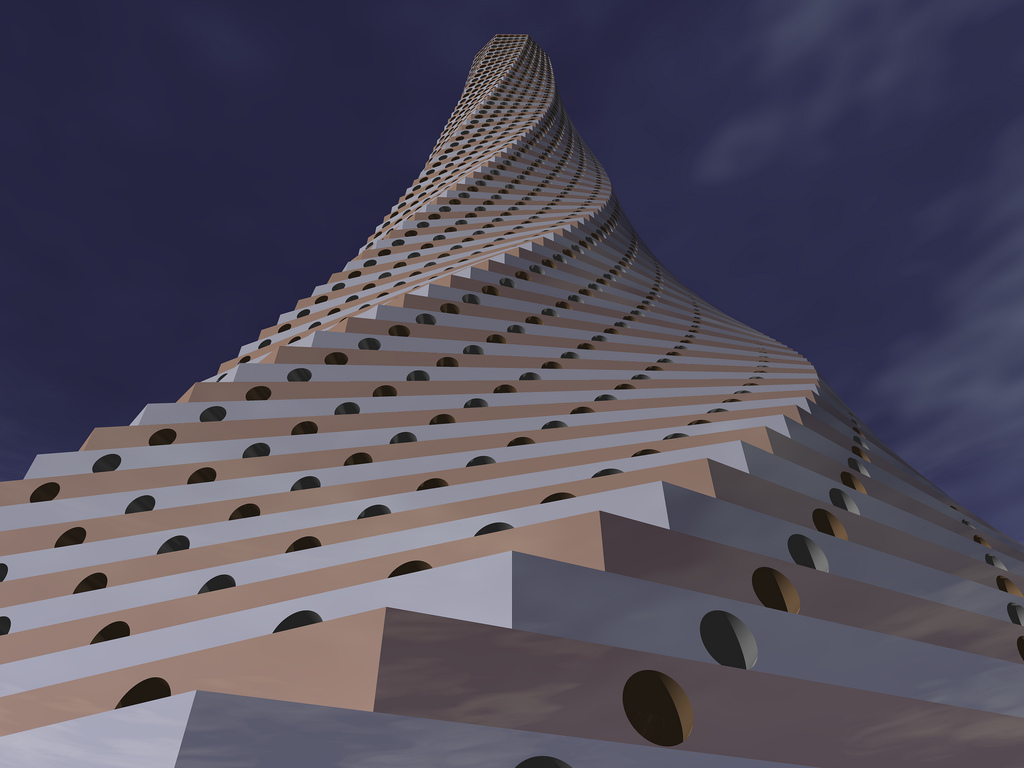
\includegraphics[width=0.85\textwidth, keepaspectratio=true]{images/introduction.jpg}
  \end{figure}
\end{frame}

\begin{frame}{Introduction}{Overview}
  \begin{figure}[overview]
    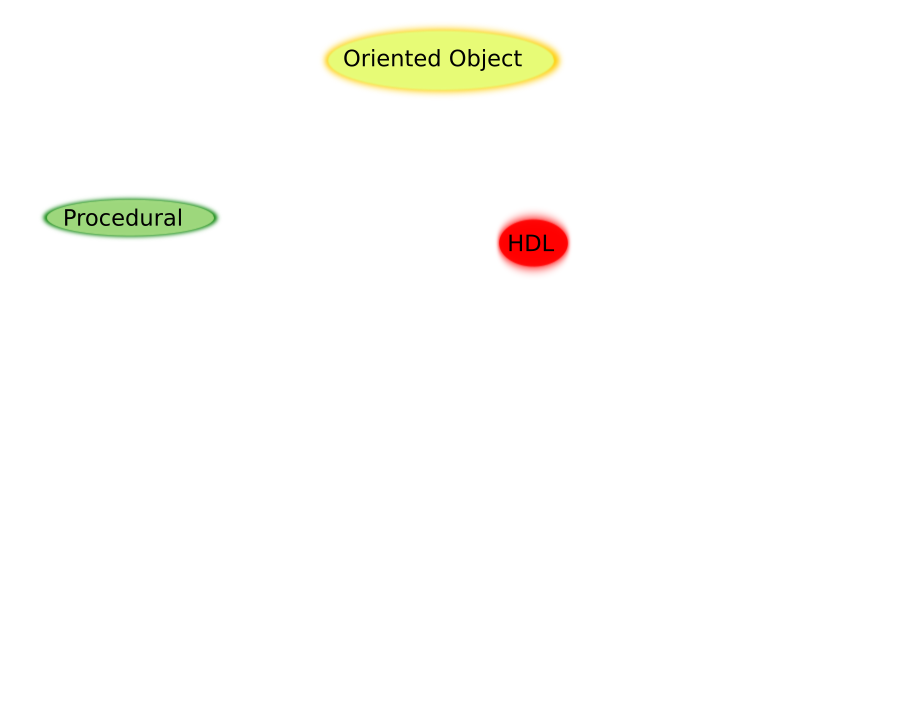
\includegraphics[width=0.7\textwidth]{images/paradigms.png}
  \end{figure}
\end{frame}

\begin{frame}{Introduction}{Overview}
  \begin{figure}[overview]
    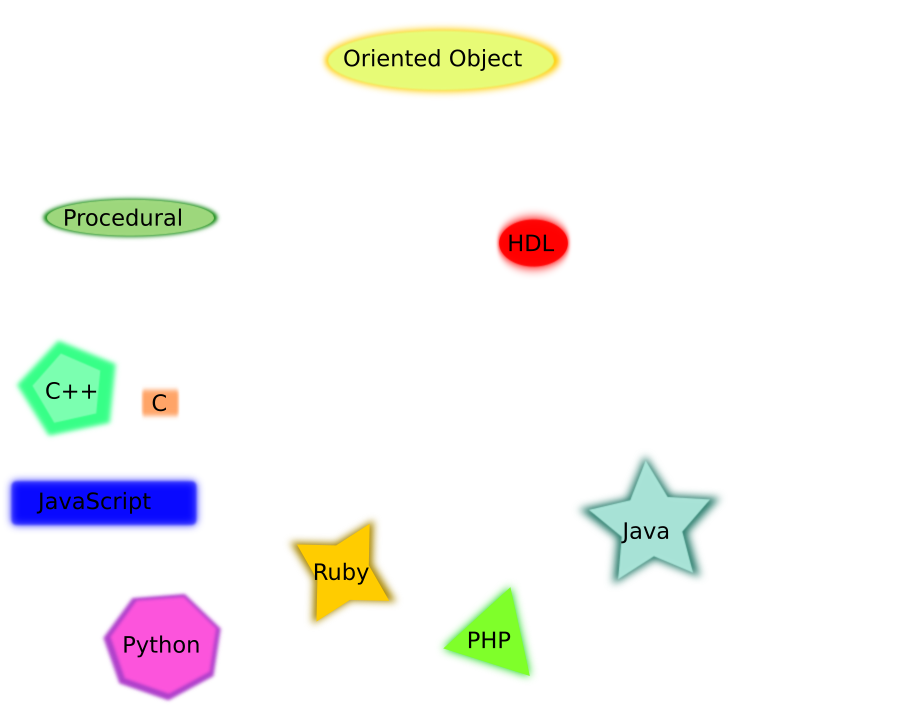
\includegraphics[width=0.7\textwidth]{images/paradigmAndLanguages.png}
  \end{figure}
\end{frame}

\begin{frame}{Introduction}{Overview}
  \begin{figure}[overview]
    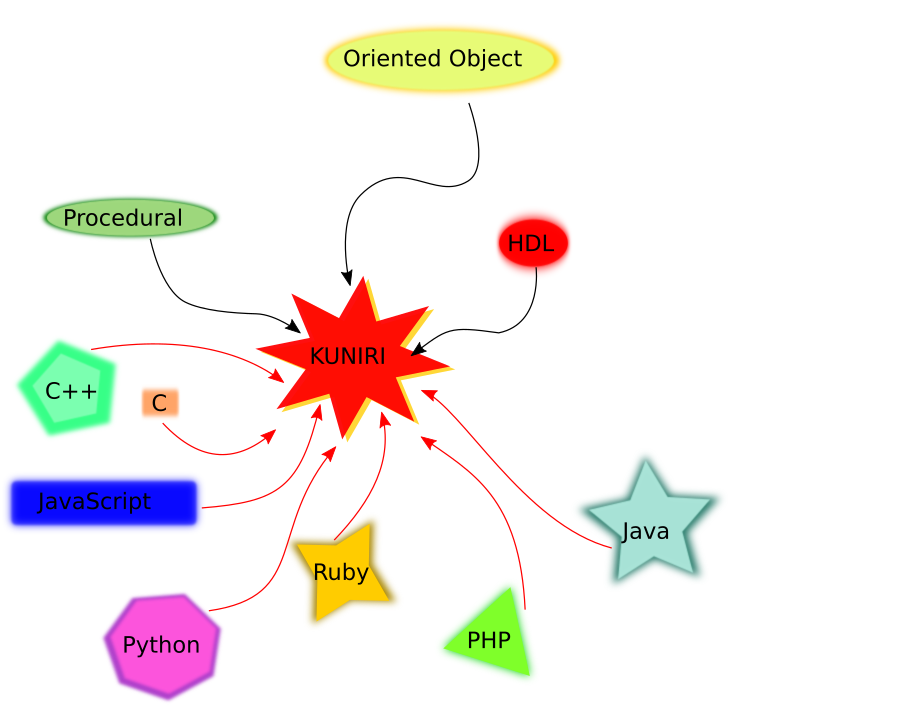
\includegraphics[width=0.7\textwidth]{images/paradigmAndLanguagesAndKuniri.png}
  \end{figure}
\end{frame}

\begin{frame}{Introduction}{Overview}
  \begin{figure}[overview]
    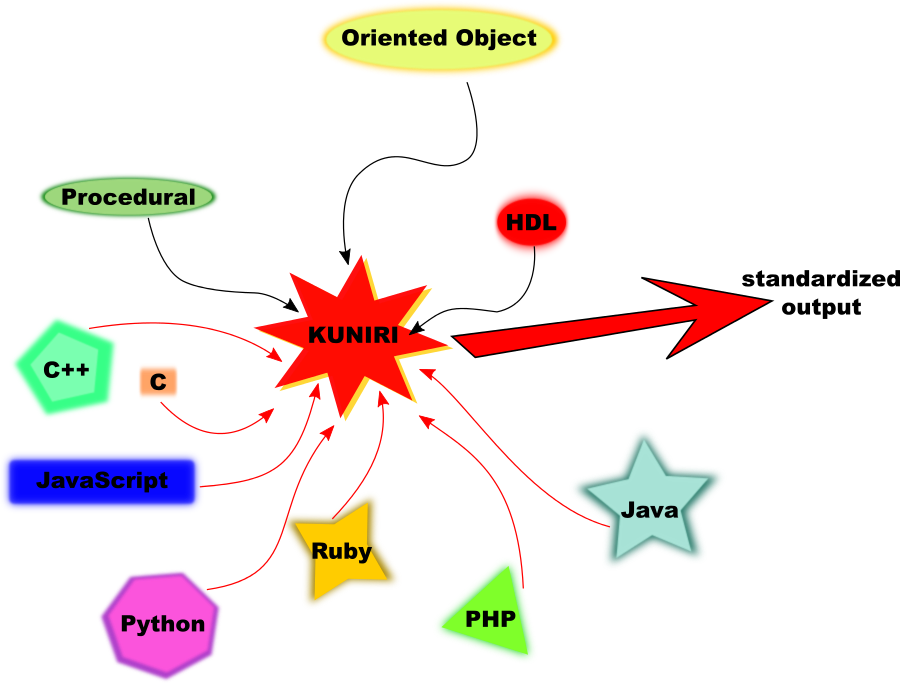
\includegraphics[width=0.7\textwidth]{images/overview.png}
  \end{figure}
\end{frame}

%-------------------------------------------------------
\begin{frame}{Introduction}{History}

  \begin{columns}
  \begin{column}{0.4\textwidth}
    \begin{figure}[fga]
      
\includegraphics[width=0.8\textwidth]{images/fga.png}
    \end{figure}
  \end{column}

  \begin{column}{0.4\textwidth}
    \begin{figure}[paulo]
      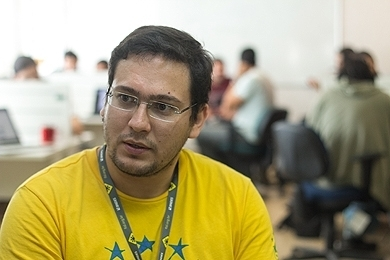
\includegraphics[width=1.2\textwidth]{images/prmm.jpg}
    \end{figure}
  \end{column}
  \end{columns}

\end{frame}

%-------------------------------------------------------
\begin{frame}{Introduction}{About our logo}
  \begin{figure}[overview]
    
\includegraphics[width=0.68\textwidth]{images/2.jpg}
  \end{figure}
\end{frame}

%-------------------------------------------------------
\begin{frame}{Introduction}{About our organization}
  \begin{figure}[overview]
    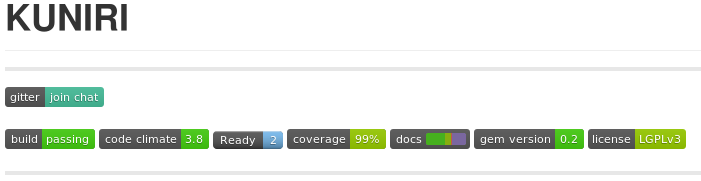
\includegraphics[width=0.7\textwidth]{images/github.png}
  \end{figure}
\end{frame}

\begin{frame}{Introduction}{About our organization}
  \begin{figure}[overview]
    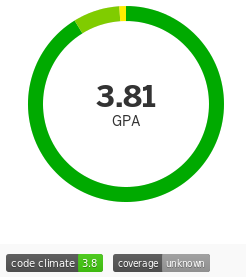
\includegraphics[width=0.5\textwidth]{images/codeclimate.png}
  \end{figure}
\end{frame}

\begin{frame}{Introduction}{About our organization}
  \begin{figure}[overview]
    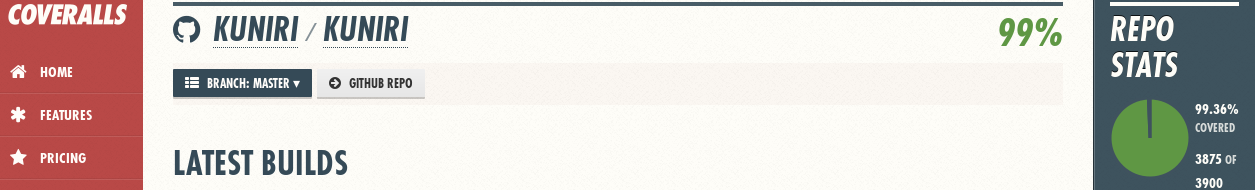
\includegraphics[width=0.8\textwidth]{images/coveralls.png}
  \end{figure}
\end{frame}

\begin{frame}{Introduction}{About our organization}
  \begin{figure}[overview]
    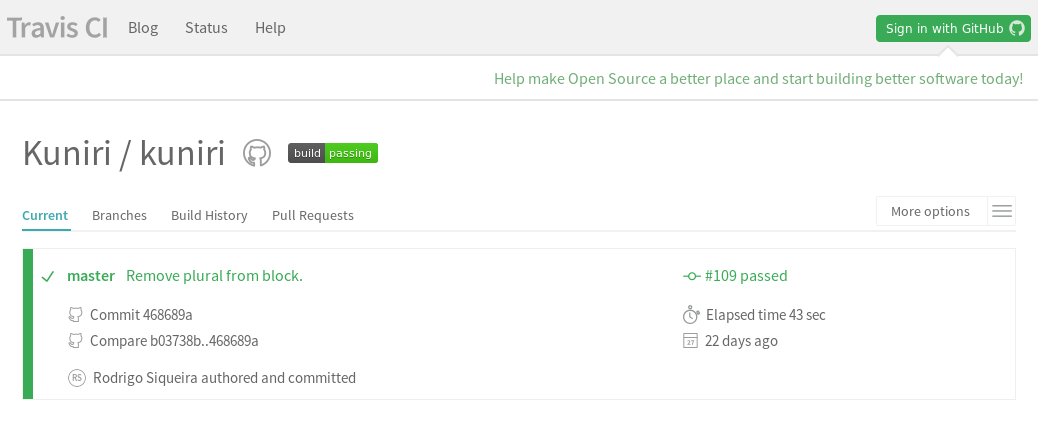
\includegraphics[width=0.9\textwidth]{images/travisci.png}
  \end{figure}
\end{frame}

\begin{frame}{Introduction}{About our organization}
  \begin{figure}[overview]
    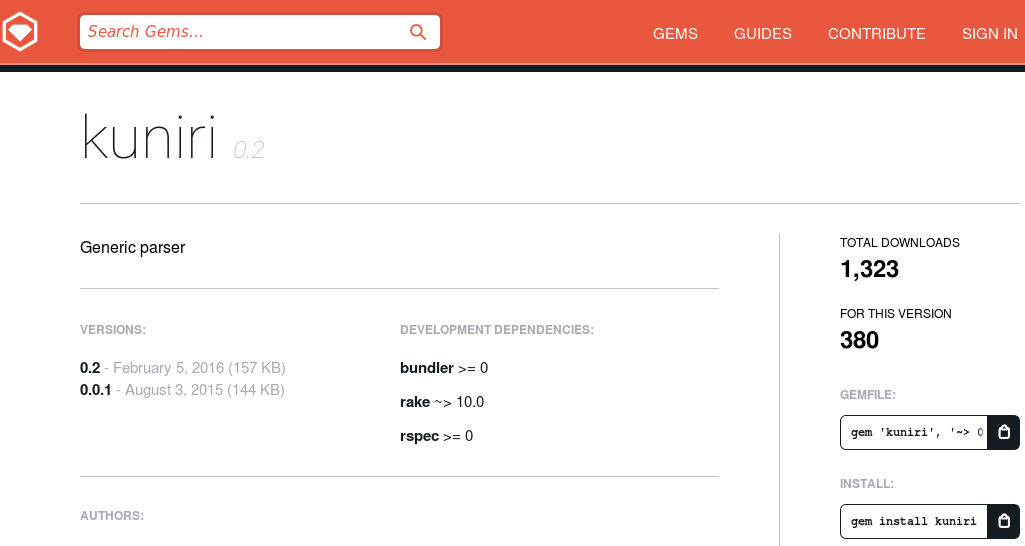
\includegraphics[width=0.8\textwidth]{images/rubygems.png}
  \end{figure}
\end{frame}

%=======================================================
\section{Kuniri Architecture}
%=======================================================
\begin{frame}{Architecture}{Overview}
  \begin{figure}[overview]
    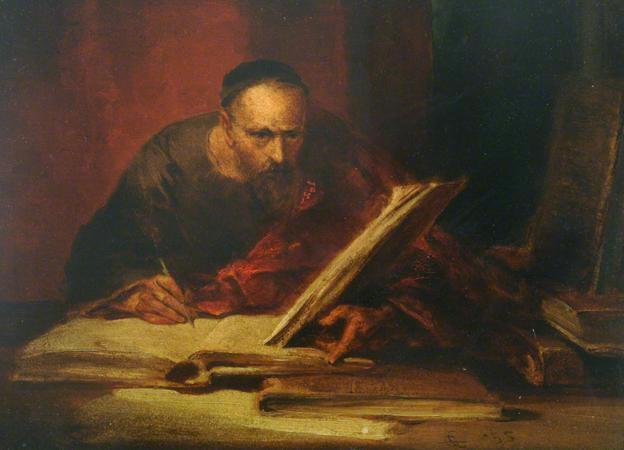
\includegraphics[width=0.7\textwidth]{images/scribe_cattermole.jpg}
  \end{figure}
\end{frame}

\begin{frame}[fragile]{Architecture}{Overview - ruby}
  Ruby Code
  \begin{columns}
    \begin{column}{0.6\textwidth}
      \small
\begin{lstlisting}
class MasterClass
  @attrTest
  def initialize
    ...
  end
  def validateInput
    ...
  end
end
\end{lstlisting}
    \end{column}

    \begin{column}{0.4\textwidth}
      Class name: \textcolor{red}{MasterClass}\\ \pause
      Attributes: \textcolor{red}{attrTest}\\ \pause
      Constructor: \textcolor{red}{initialize}\\ \pause
      Methods: \textcolor{red}{validateInput}\\
    \end{column}

  \end{columns}
\end{frame}

\begin{frame}[fragile]{Architecture}{Overview - Java}
  \begin{columns}
    \begin{column}{0.6\textwidth}
      \small
\begin{lstlisting}
class XptoClass{
  private int value;
  XptoClass(){
    ...
  }
  public void validateXpto(){
    ...
  }
}
\end{lstlisting}
    \end{column}

    \begin{column}{0.4\textwidth}
      Class name: \textcolor{red}{XptoClass}\\ \pause
      Attributes: \textcolor{red}{value}\\ \pause
      Constructor: \textcolor{red}{XptoClass}\\ \pause
      Methods: \textcolor{red}{validateXpto}\\
    \end{column}

  \end{columns}
\end{frame}

%-------------------------------------------------------
\begin{frame}{Architecture}{All}
  \begin{figure}[all]
    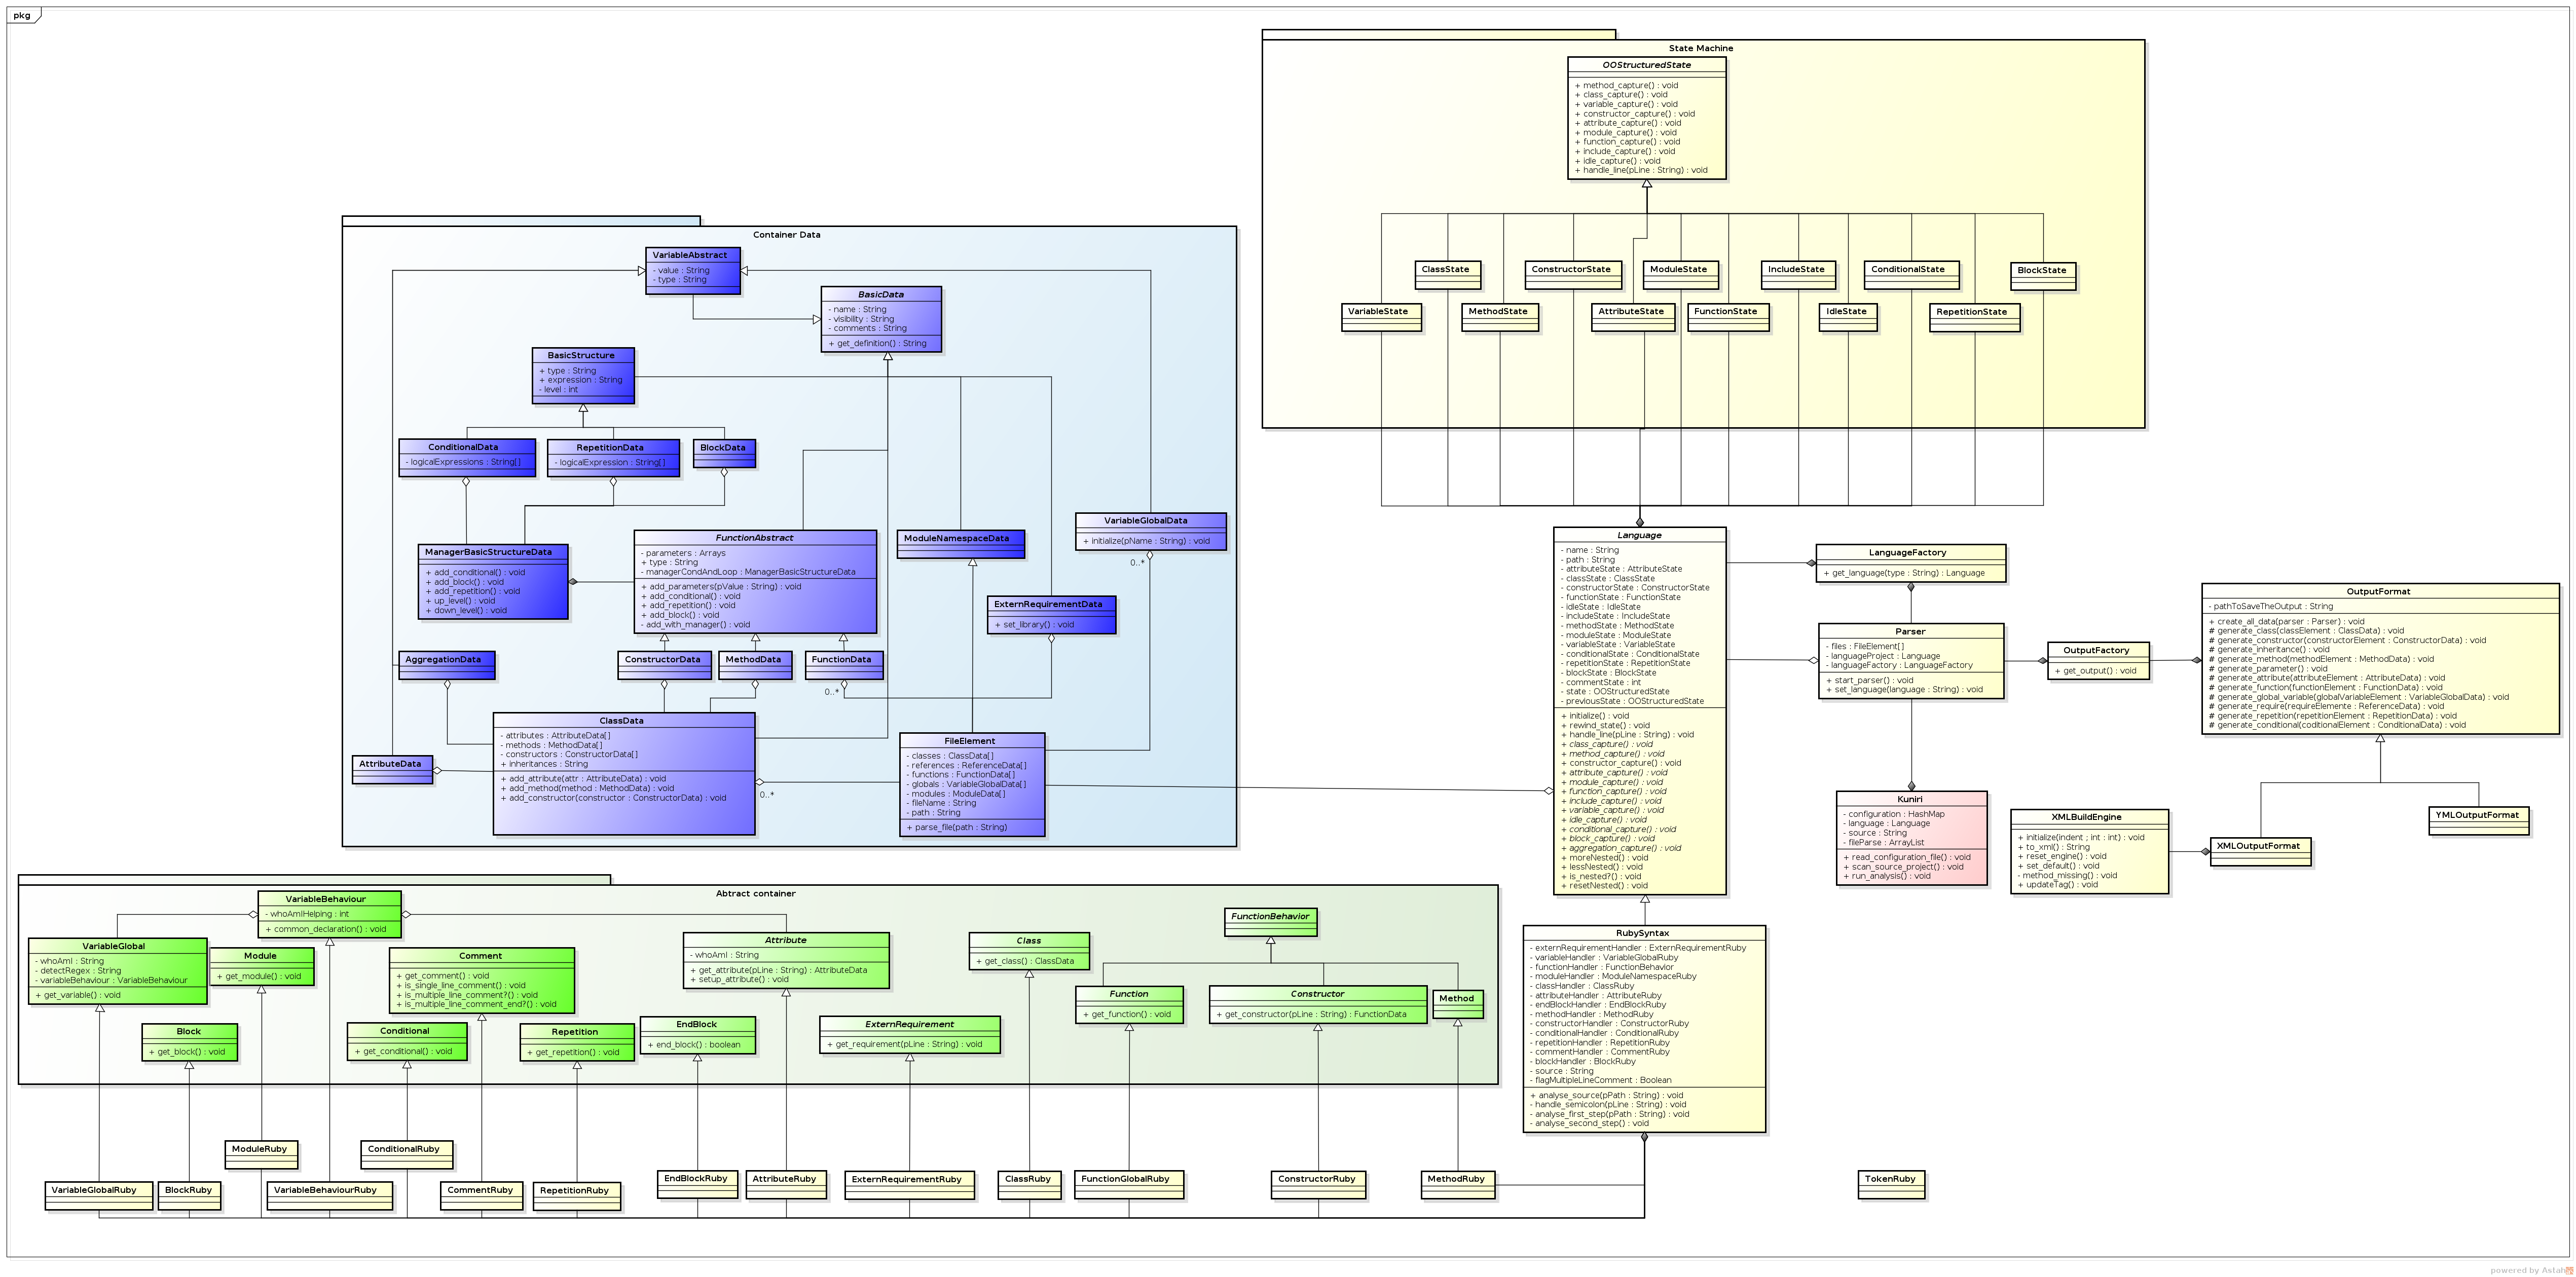
\includegraphics[width=0.97\textwidth]{images/OverviewClasses.png}
  \end{figure}
\end{frame}

\begin{frame}{Architecture}{Container Data}
  \begin{figure}[containerdata]
    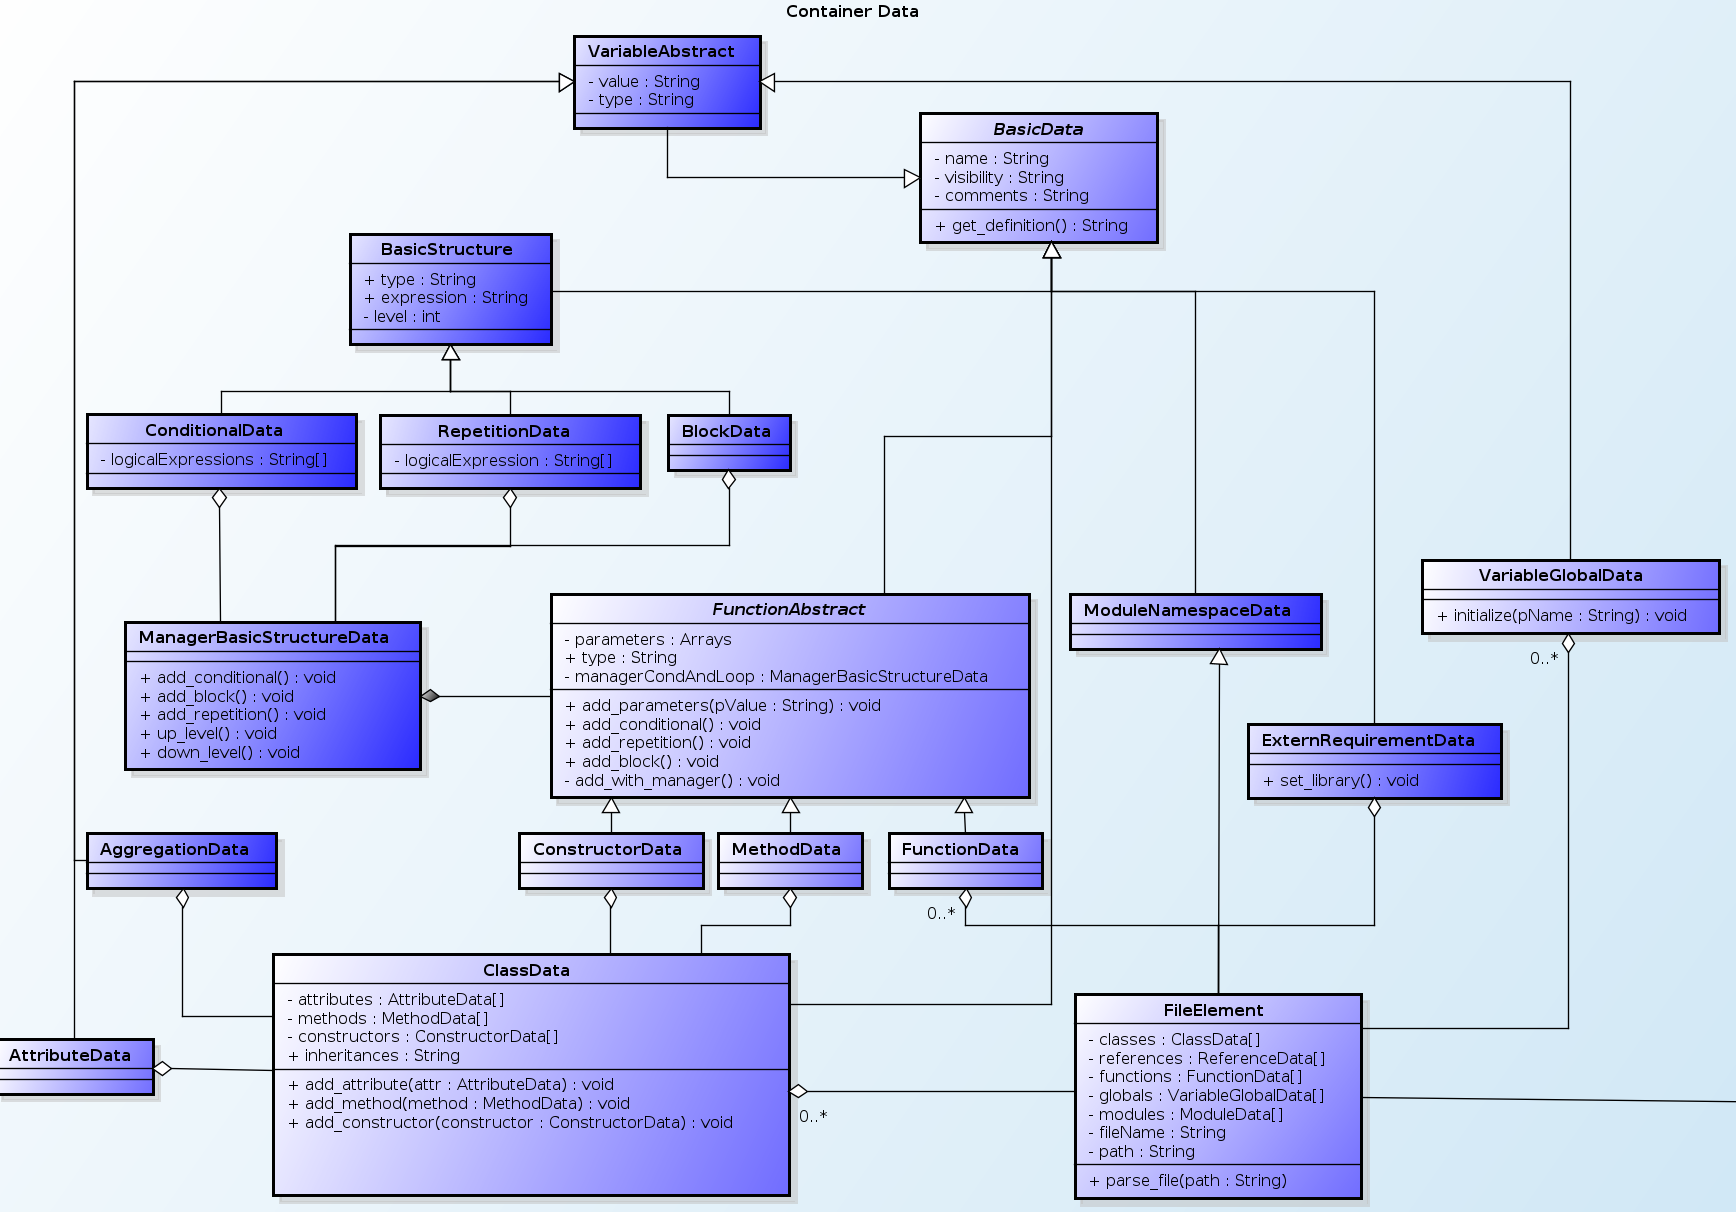
\includegraphics[width=0.93\textwidth]{images/ContainerData.png}
  \end{figure}
\end{frame}

\begin{frame}{Architecture}{Container Data}
  \begin{figure}[classAndFileElement]
    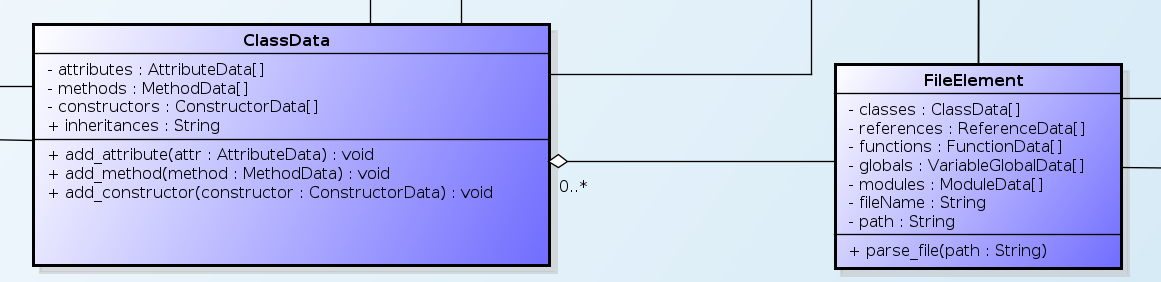
\includegraphics[width=0.9\textwidth]{images/classAndFileElementData.png}
  \end{figure}
\end{frame}

\begin{frame}{Architecture}{Container Data}
  \begin{figure}[overview]
    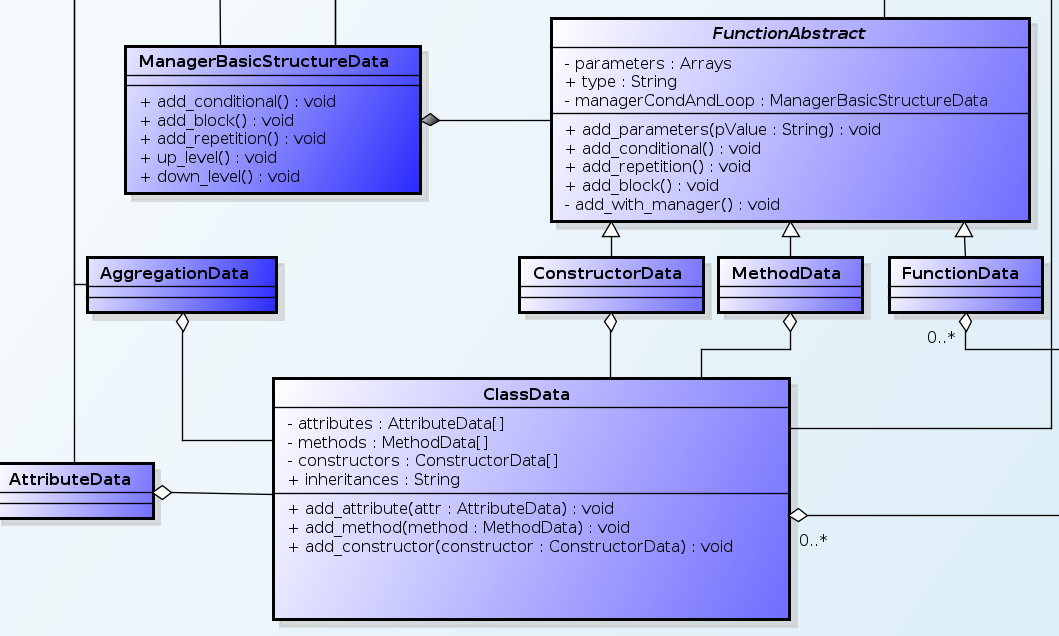
\includegraphics[width=0.9\textwidth]{images/functionBehaviour.png}
  \end{figure}
\end{frame}


%-------------------------------------------------------
\begin{frame}{Architecture}{Abstract Container}
  \begin{figure}[overview]
    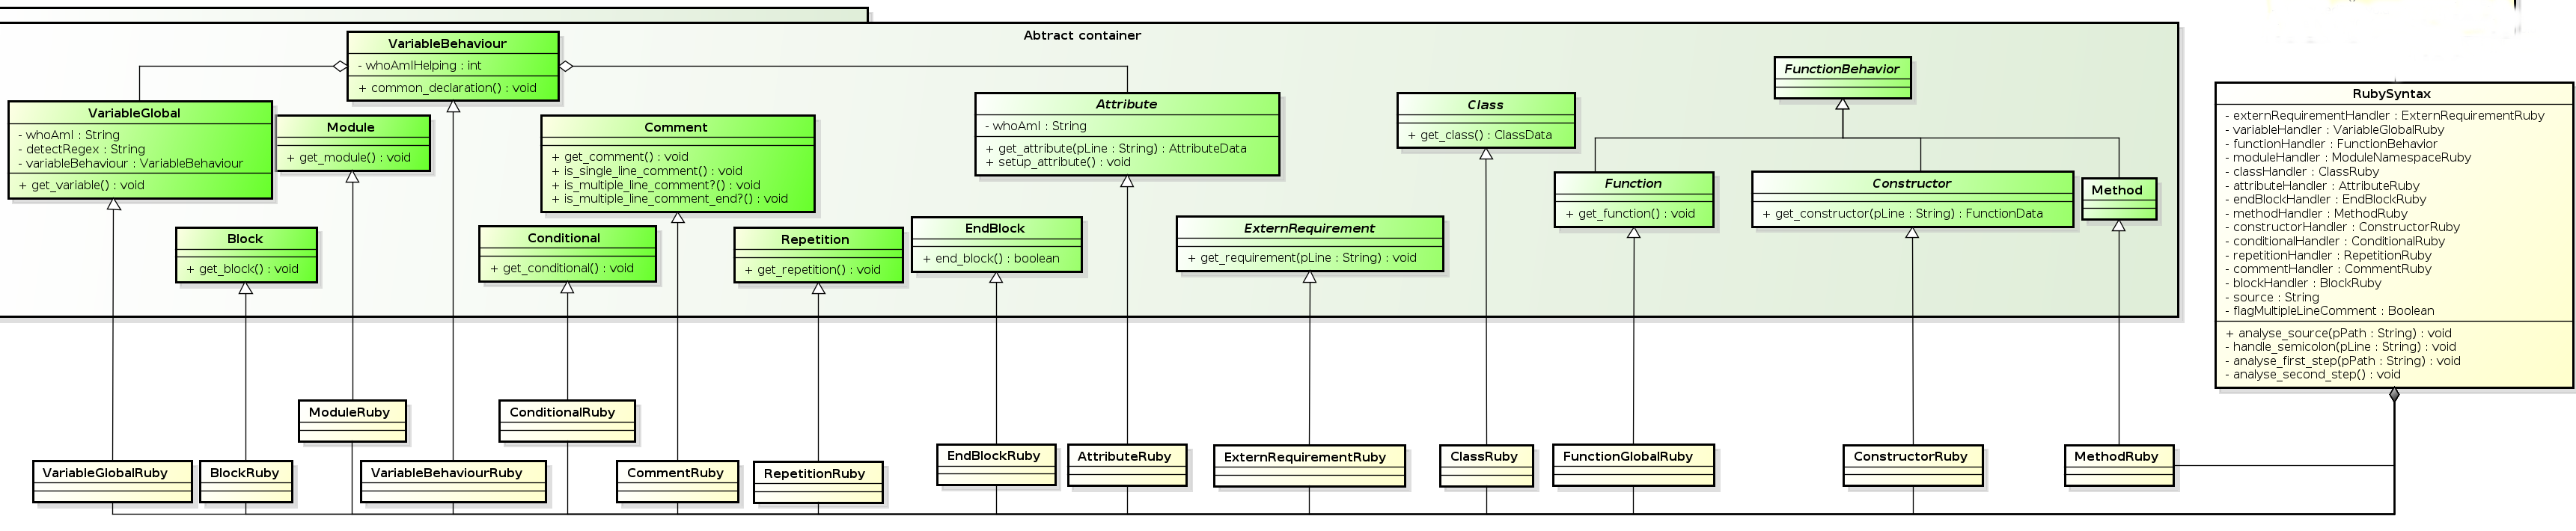
\includegraphics[width=1\textwidth]{images/abstractContainer.png}
  \end{figure}
\end{frame}

\begin{frame}{Architecture}{Strategy - GoF pattern}
  \begin{figure}[stategof]
    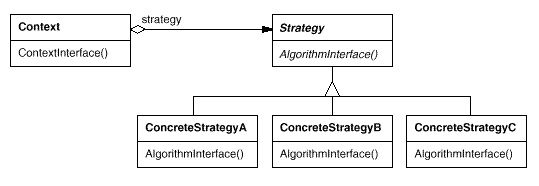
\includegraphics[width=0.9\textwidth]{images/strategy.png}
  \end{figure}
\end{frame}

\begin{frame}{Architecture}{Abstract Container}
  \begin{figure}[overview]
    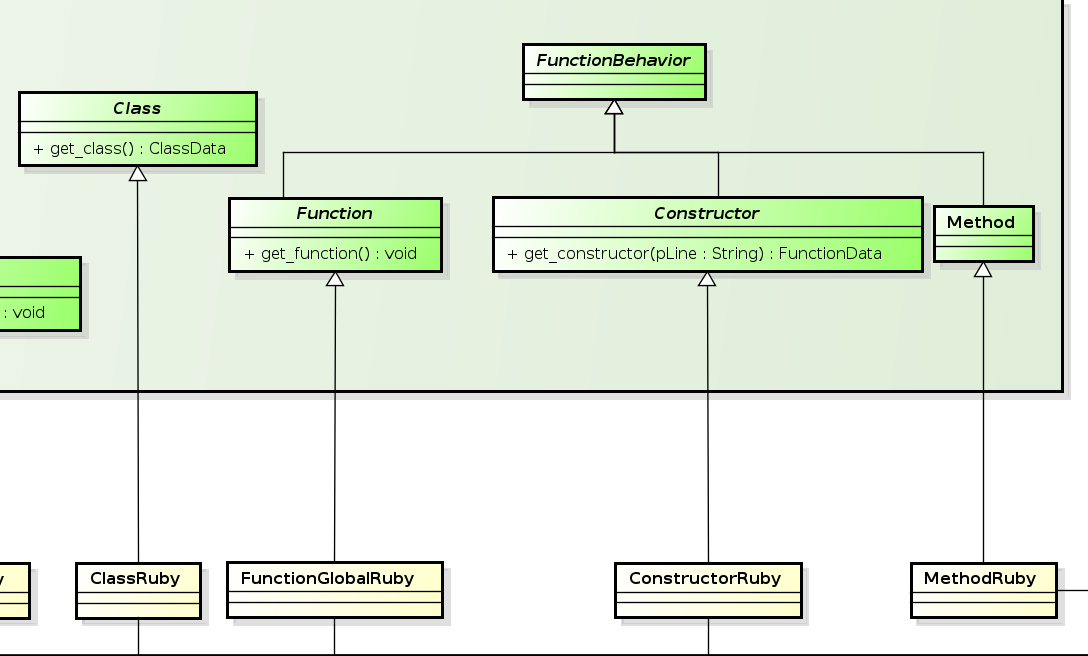
\includegraphics[width=0.9\textwidth]{images/abstractContainerClasses.png}
  \end{figure}
\end{frame}

\begin{frame}{Architecture}{Abstract Container}
  \begin{figure}[overview]
    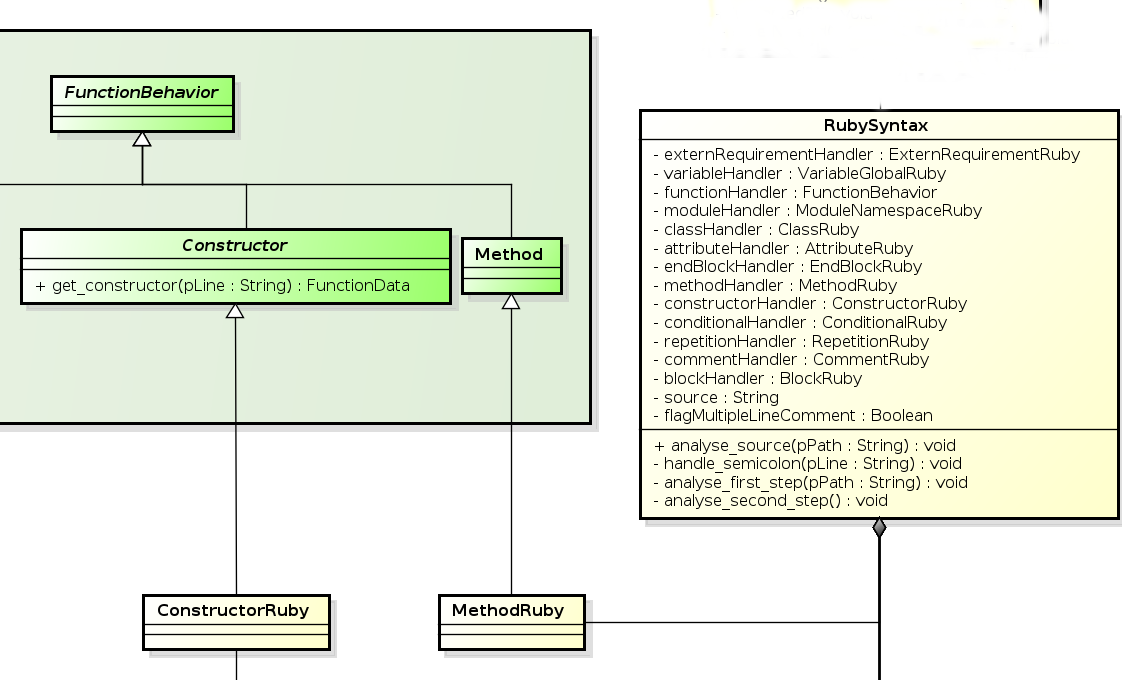
\includegraphics[width=0.9\textwidth]{images/abstractContainerConcrete.png}
  \end{figure}
\end{frame}

\begin{frame}[fragile]{Simple Code}{Demonstration}
Code from: lib/kuniri/language/ruby/class\_ruby.rb
\small
\begin{lstlisting}
...
class ClassRuby < Languages::Class
  ...
  def get_class(pLine)
    result = detect_class(pLine)
    return nil unless result

    classCaptured = Languages::ClassData.new
    ...
    return classCaptured
  end
  ...
  def detect_class(pLine)
    regexExpression = /^\s*class\s+(.*)/
    ...
  end
...
\end{lstlisting}
\end{frame}

%-------------------------------------------------------
\begin{frame}{Architecture}{State Machine}
  \begin{figure}[All]
    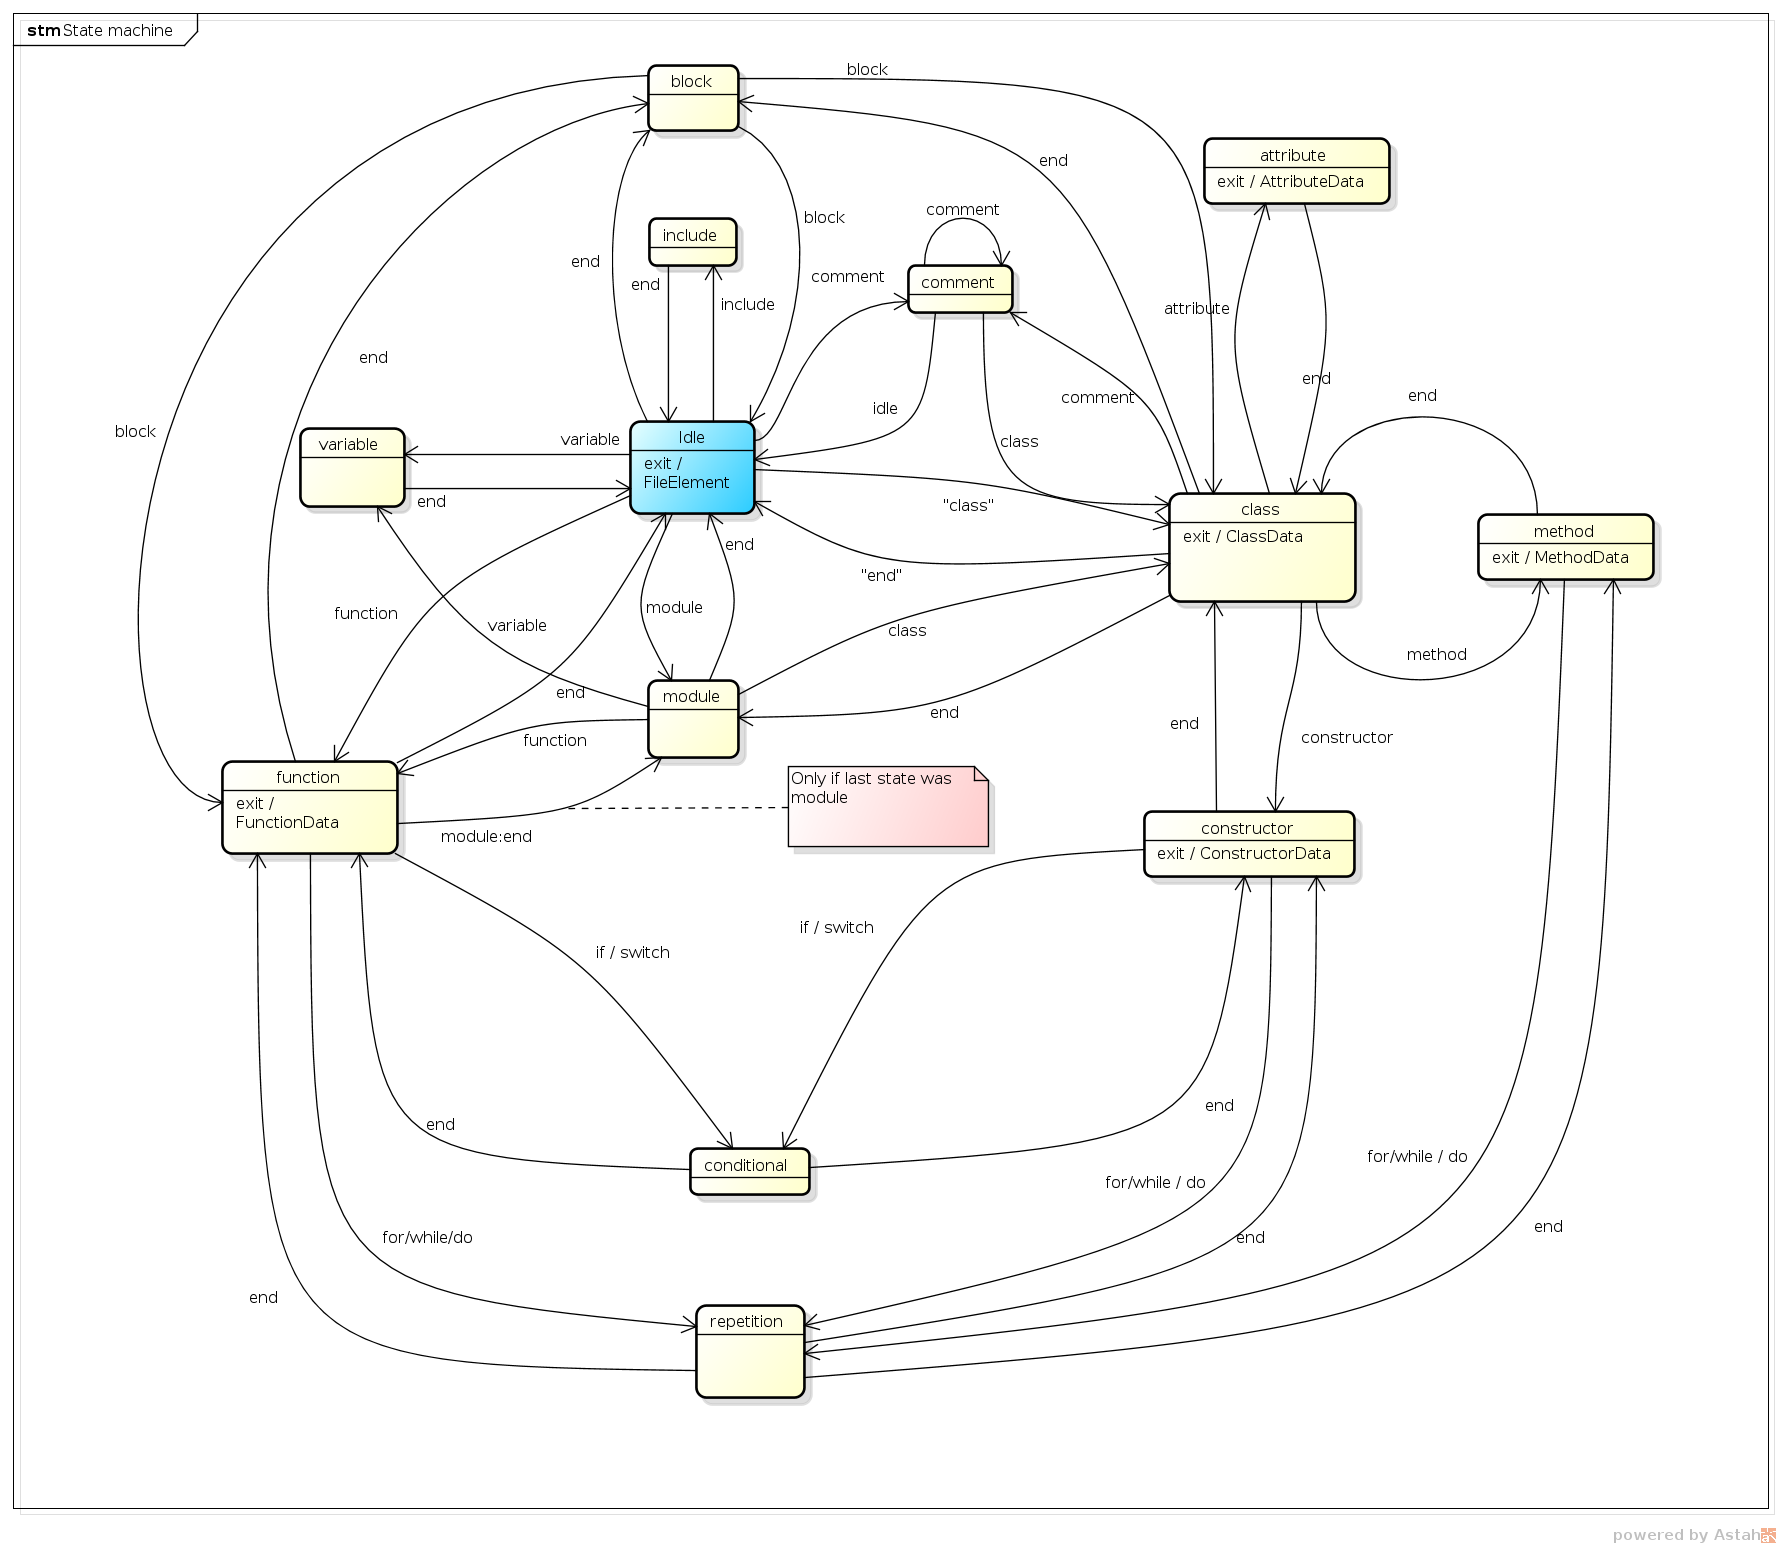
\includegraphics[width=0.8\textwidth]{images/fsm.png}
  \end{figure}
\end{frame}

\begin{frame}{Architecture}{State Machine - GoF pattern}
  \begin{figure}[stategof]
    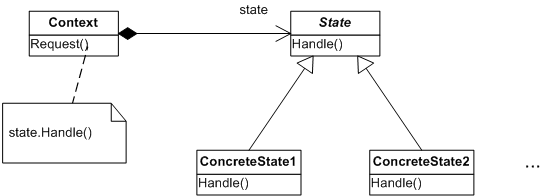
\includegraphics[width=0.8\textwidth]{images/state.png}
  \end{figure}
\end{frame}

\begin{frame}{Architecture}{State Machine}
  \begin{figure}[All]
    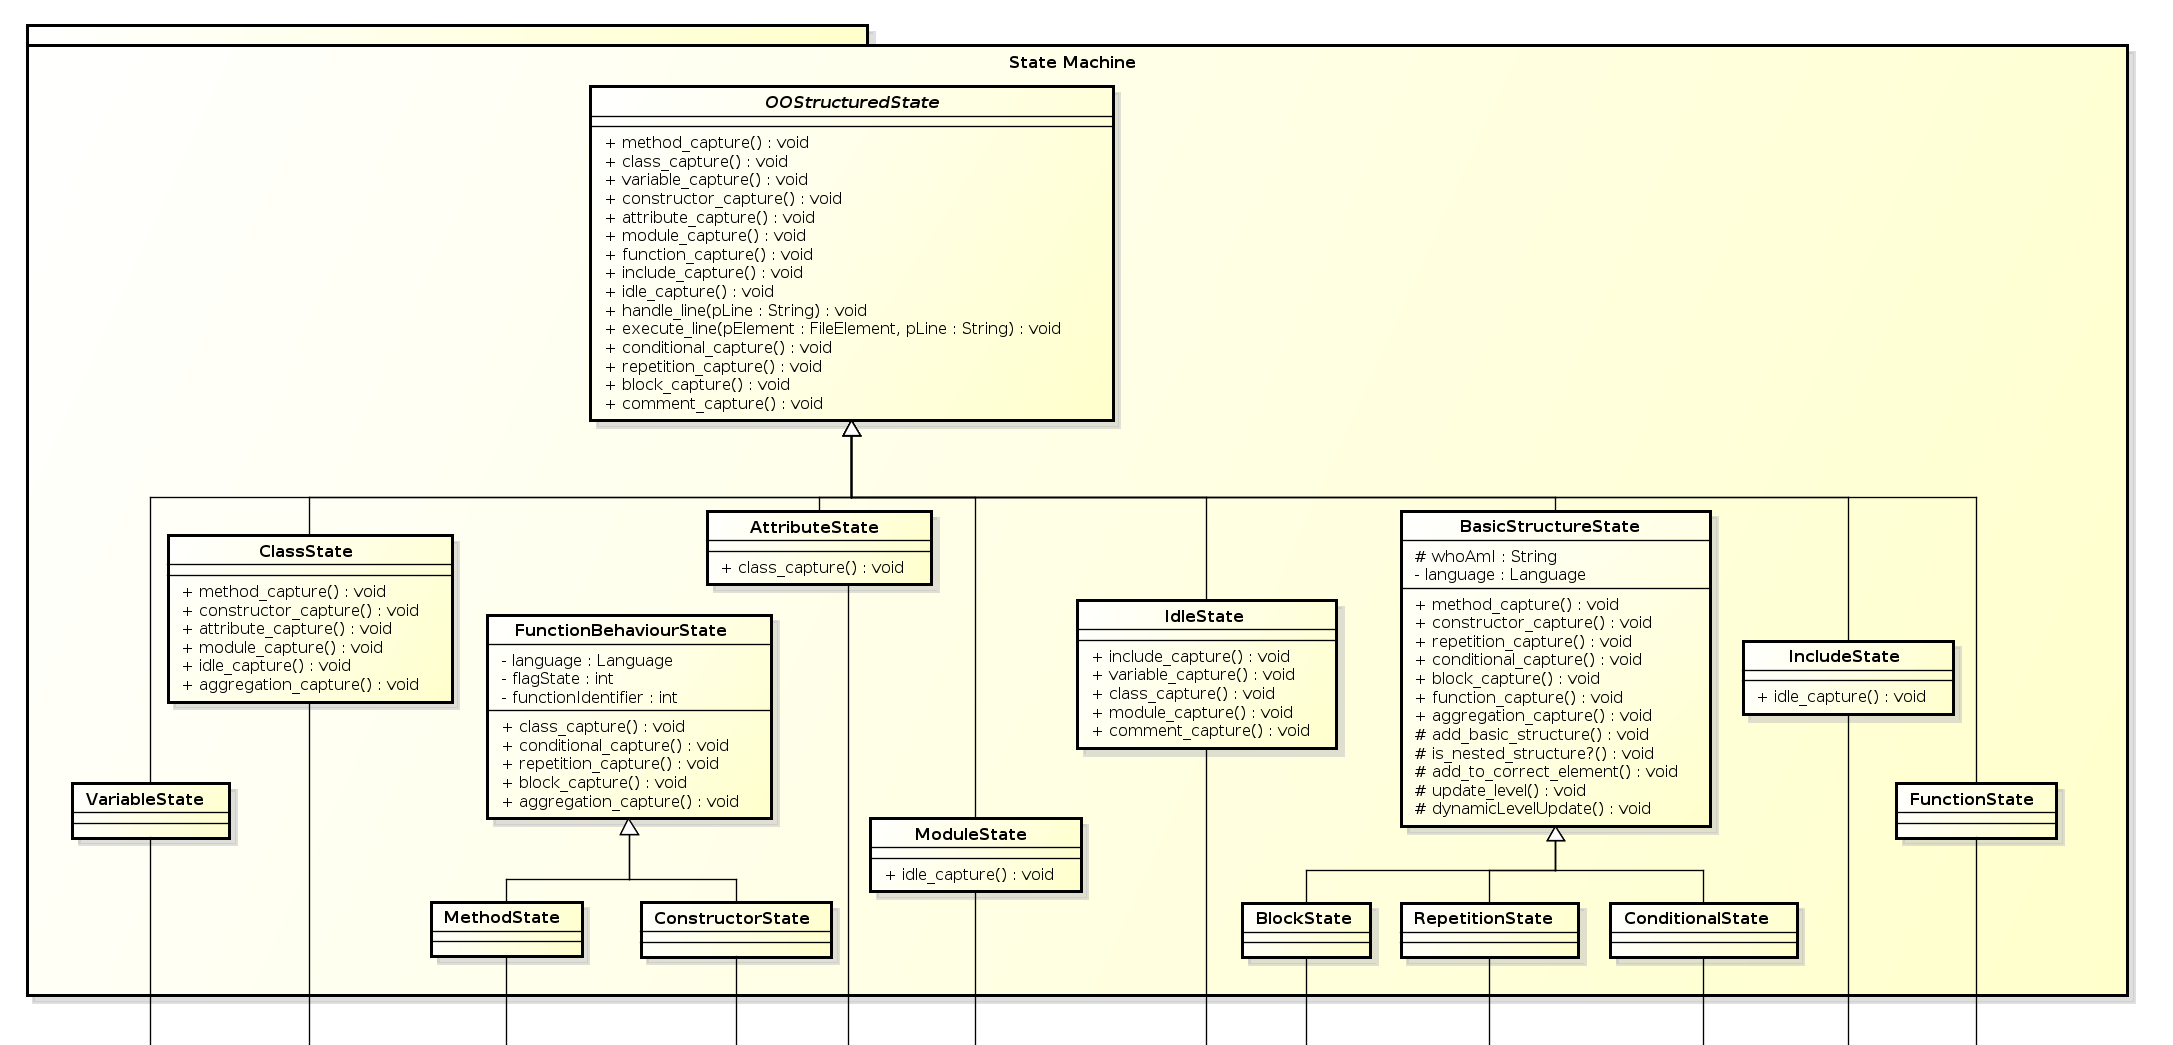
\includegraphics[width=0.9\textwidth]{images/fsmPack.png}
  \end{figure}
\end{frame}

\begin{frame}{Architecture}{State Machine}
  \begin{figure}[Look at FSM]
    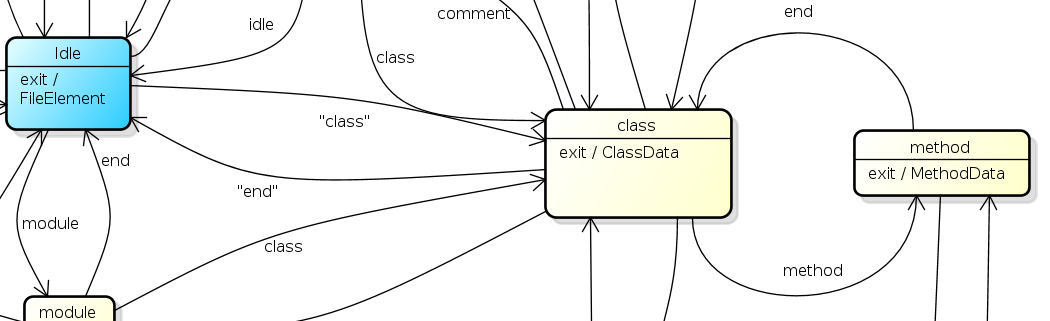
\includegraphics[width=0.9\textwidth]{images/idleToClassToMethod.png}
  \end{figure}
\end{frame}

\begin{frame}{Architecture}{State Machine}
  \begin{figure}[Look at class structure]
    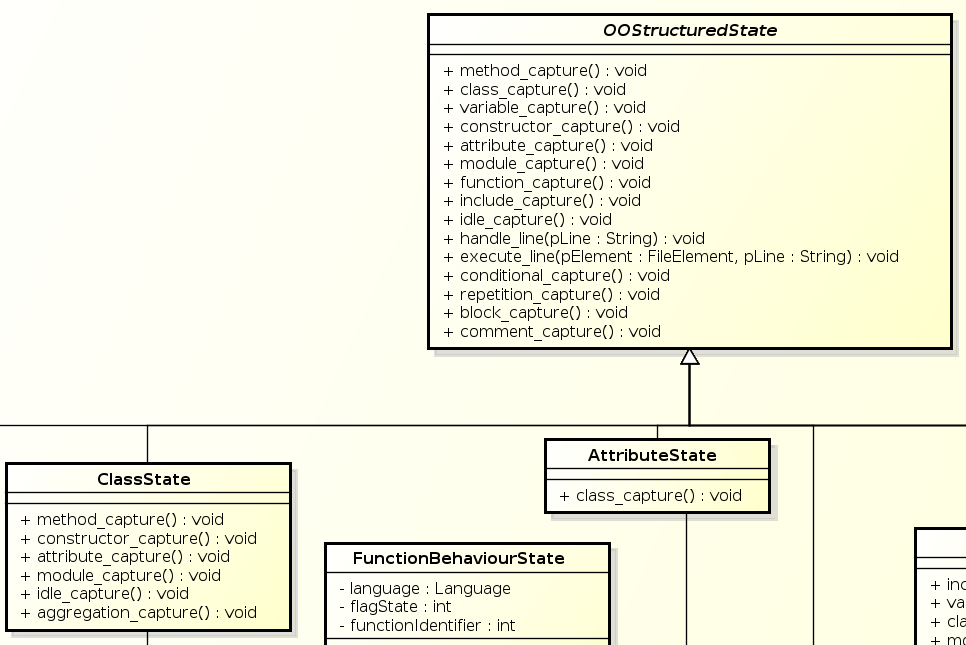
\includegraphics[width=0.9\textwidth]{images/classFSM.png}
  \end{figure}
\end{frame}

\begin{frame}[fragile]{Simple Code}{Demonstration}
Code from: lib/kuniri/state\_machine/OO\_structured\_fsm/class\_state.rb
\small
\begin{lstlisting}
...
class ClassState < OOStructuredState
  @language
  def initialize (pLanguage)
    @language = pLanguage
  end
  def handle_line(pLine)
    if @language.line_inspect(AGGREGATION_ID, pLine)
      aggregation_capture
  ...
  end
  def method_capture
    @language.set_state(@language.methodState)
  end
...
\end{lstlisting}
\end{frame}

%-------------------------------------------------------

%=======================================================
\section{Law of Demeter inside Kuniri}
%=======================================================
\begin{frame}{Law of Demeter}{Overview}
\begin{block}{Law Of Demeter}
A method of an object should invoke only the methods of the following kinds of
objects:
  \begin{enumerate}
    \item itself
    \item its parameters
    \item any objects it creates/instantiates
    \item its direct component objects
  \end{enumerate}
\end{block}
\end{frame}

\begin{frame}{Architecture}{Law of Demeter}
  \begin{figure}[Look at class structure]
    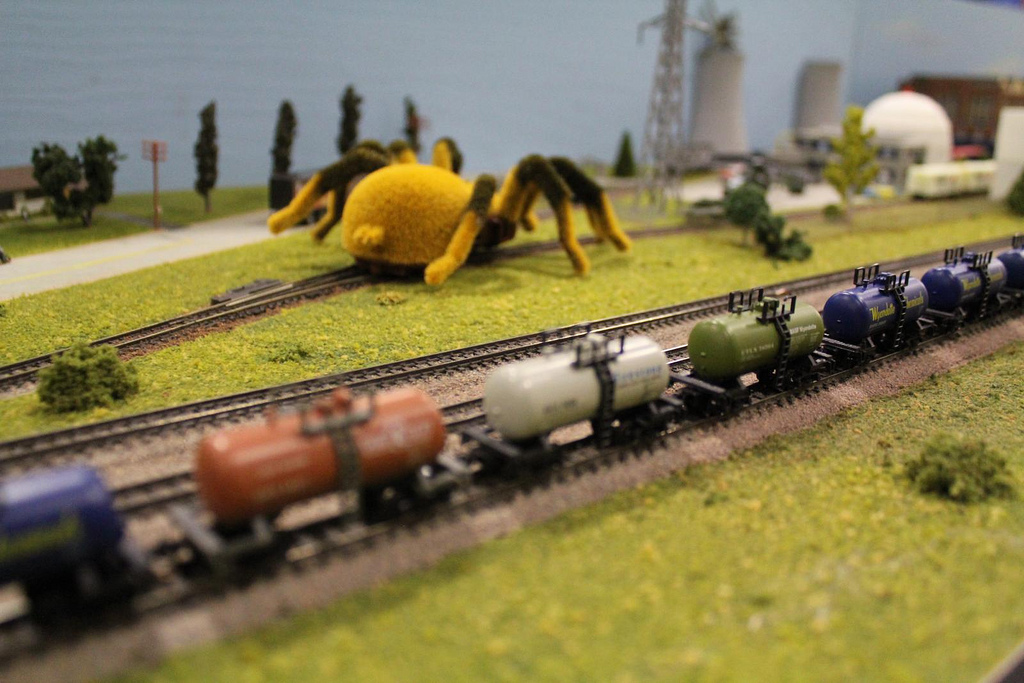
\includegraphics[width=0.8\textwidth]{images/demeter_train.jpg}
  \end{figure}
\end{frame}

%-------------------------------------------------------
\begin{frame}[fragile]{Law of Demeter}{Real code}
Code from: lib/kuniri/state\_machine/OO\_structured\_fsm/class\_state.rb
\small
\begin{lstlisting}
...
def execute(pElementFile, pLine)
  attributeElement = @language.attributeHandler.get_attribute(pLine)
  if attributeElement
    lastIndex = pElementFile.classes.length - 1
    attributeElement.each do |attribute|
      attribute.comments = @language.string_comment_to_transfer
    end
    @language.string_comment_to_transfer = ''
    pElementFile.classes[lastIndex].add_attribute(attributeElement)
  end
...
\end{lstlisting}
\end{frame}

\begin{frame}[fragile]{Law of Demeter}{Apply LoD}
Code from:
lib/kuniri/language/container\_data/structured\_and\_oo/
\small
\begin{lstlisting}
...
class FileElementData < Languages::BasicData
...
 def add_attribute_to_last_class(pAttributeElement)
  classes.last.add_attribute(pAttributeElement)
 end
...
end
\end{lstlisting}
\end{frame}

\begin{frame}[fragile]{Law of Demeter}{Real code}
Code from: lib/kuniri/state\_machine/OO\_structured\_fsm/class\_state.rb
\small
\begin{lstlisting}
...
def execute(pElementFile, pLine)
  attributeElement = @language.attributeHandler.get_attribute(pLine)
  if attributeElement
    lastIndex = pElementFile.classes.length - 1
    attributeElement.each do |attribute|
      attribute.comments = @language.string_comment_to_transfer
    end
    @language.string_comment_to_transfer = ''
    pElementFile.add_attribute_to_last_class(attributeElement)
  end
...
\end{lstlisting}
\end{frame}

\begin{frame}[fragile]{Law of Demeter}{Next part}
Code from: lib/kuniri/state\_machine/OO\_structured\_fsm/class\_state.rb
\small
\begin{lstlisting}
...
def execute(pElementFile, pLine)
  attributeElement = @language.attributeHandler.get_attribute(pLine)
  if attributeElement
...
\end{lstlisting}
\end{frame}

\begin{frame}[fragile]{Law of Demeter}{Next part}
Code from: lib/kuniri/language/language.rb
\small
\begin{lstlisting}
...
def line_inspect(pTarget, pLine)
  eval("#{pTarget}Handler.get_#{pTarget}(pLine)")
end
...
\end{lstlisting}
\end{frame}

\begin{frame}[fragile]{Law of Demeter}{Next part}
Code from: lib/kuniri/state\_machine/OO\_structured\_fsm/class\_state.rb
\small
\begin{lstlisting}
...
def execute(pElementFile, pLine)
  attributeElement = @language.line_inspect('attribute', pLine)
...
\end{lstlisting}
\end{frame}

\begin{frame}[fragile]{Law of Demeter}{Problem...}
  \begin{figure}[overview]
    
\includegraphics[width=0.8\textwidth]{images/problem.jpg}
  \end{figure}
\end{frame}

\begin{frame}[fragile]{Law of Demeter}{Next part}
\small
\begin{lstlisting}
time rake

[Coveralls] Set up the SimpleCov formatter.
[Coveralls] Using SimpleCov's default settings.
..................................................

682 examples, 0 failures

Randomized with seed 6659

real 0m7.114s
user 0m6.850s
sys 0m0.227s
\end{lstlisting}
\end{frame}

\begin{frame}[fragile]{Law of Demeter}{Change it}
\small
Code from: lib/kuniri/language/language.rb
\begin{lstlisting}
...
def line_inspect(pTarget, pLine)
  case pTarget
    when StateMachine::METHOD_ID
      return @methodHandler.get_method(pLine)
    when StateMachine::CONSTRUCTOR_ID
      return @constructorHandler.get_constructor(pLine)
...
\end{lstlisting}
\end{frame}

\begin{frame}[fragile]{Law of Demeter}{Change it again}
\small
\begin{lstlisting}
time rake

[Coveralls] Set up the SimpleCov formatter.
[Coveralls] Using SimpleCov's default settings.
..................................................

682 examples, 0 failures

Randomized with seed 36092

real 0m5.139s
user 0m4.867s
sys 0m0.230s
\end{lstlisting}
\end{frame}

%-------------------------------------------------------
\begin{frame}{Law of Demeter}{Singleton and Law of Demeter}
  \begin{columns}[T]
      \begin{column}{.5\textwidth}
    \begin{figure}[overview]
      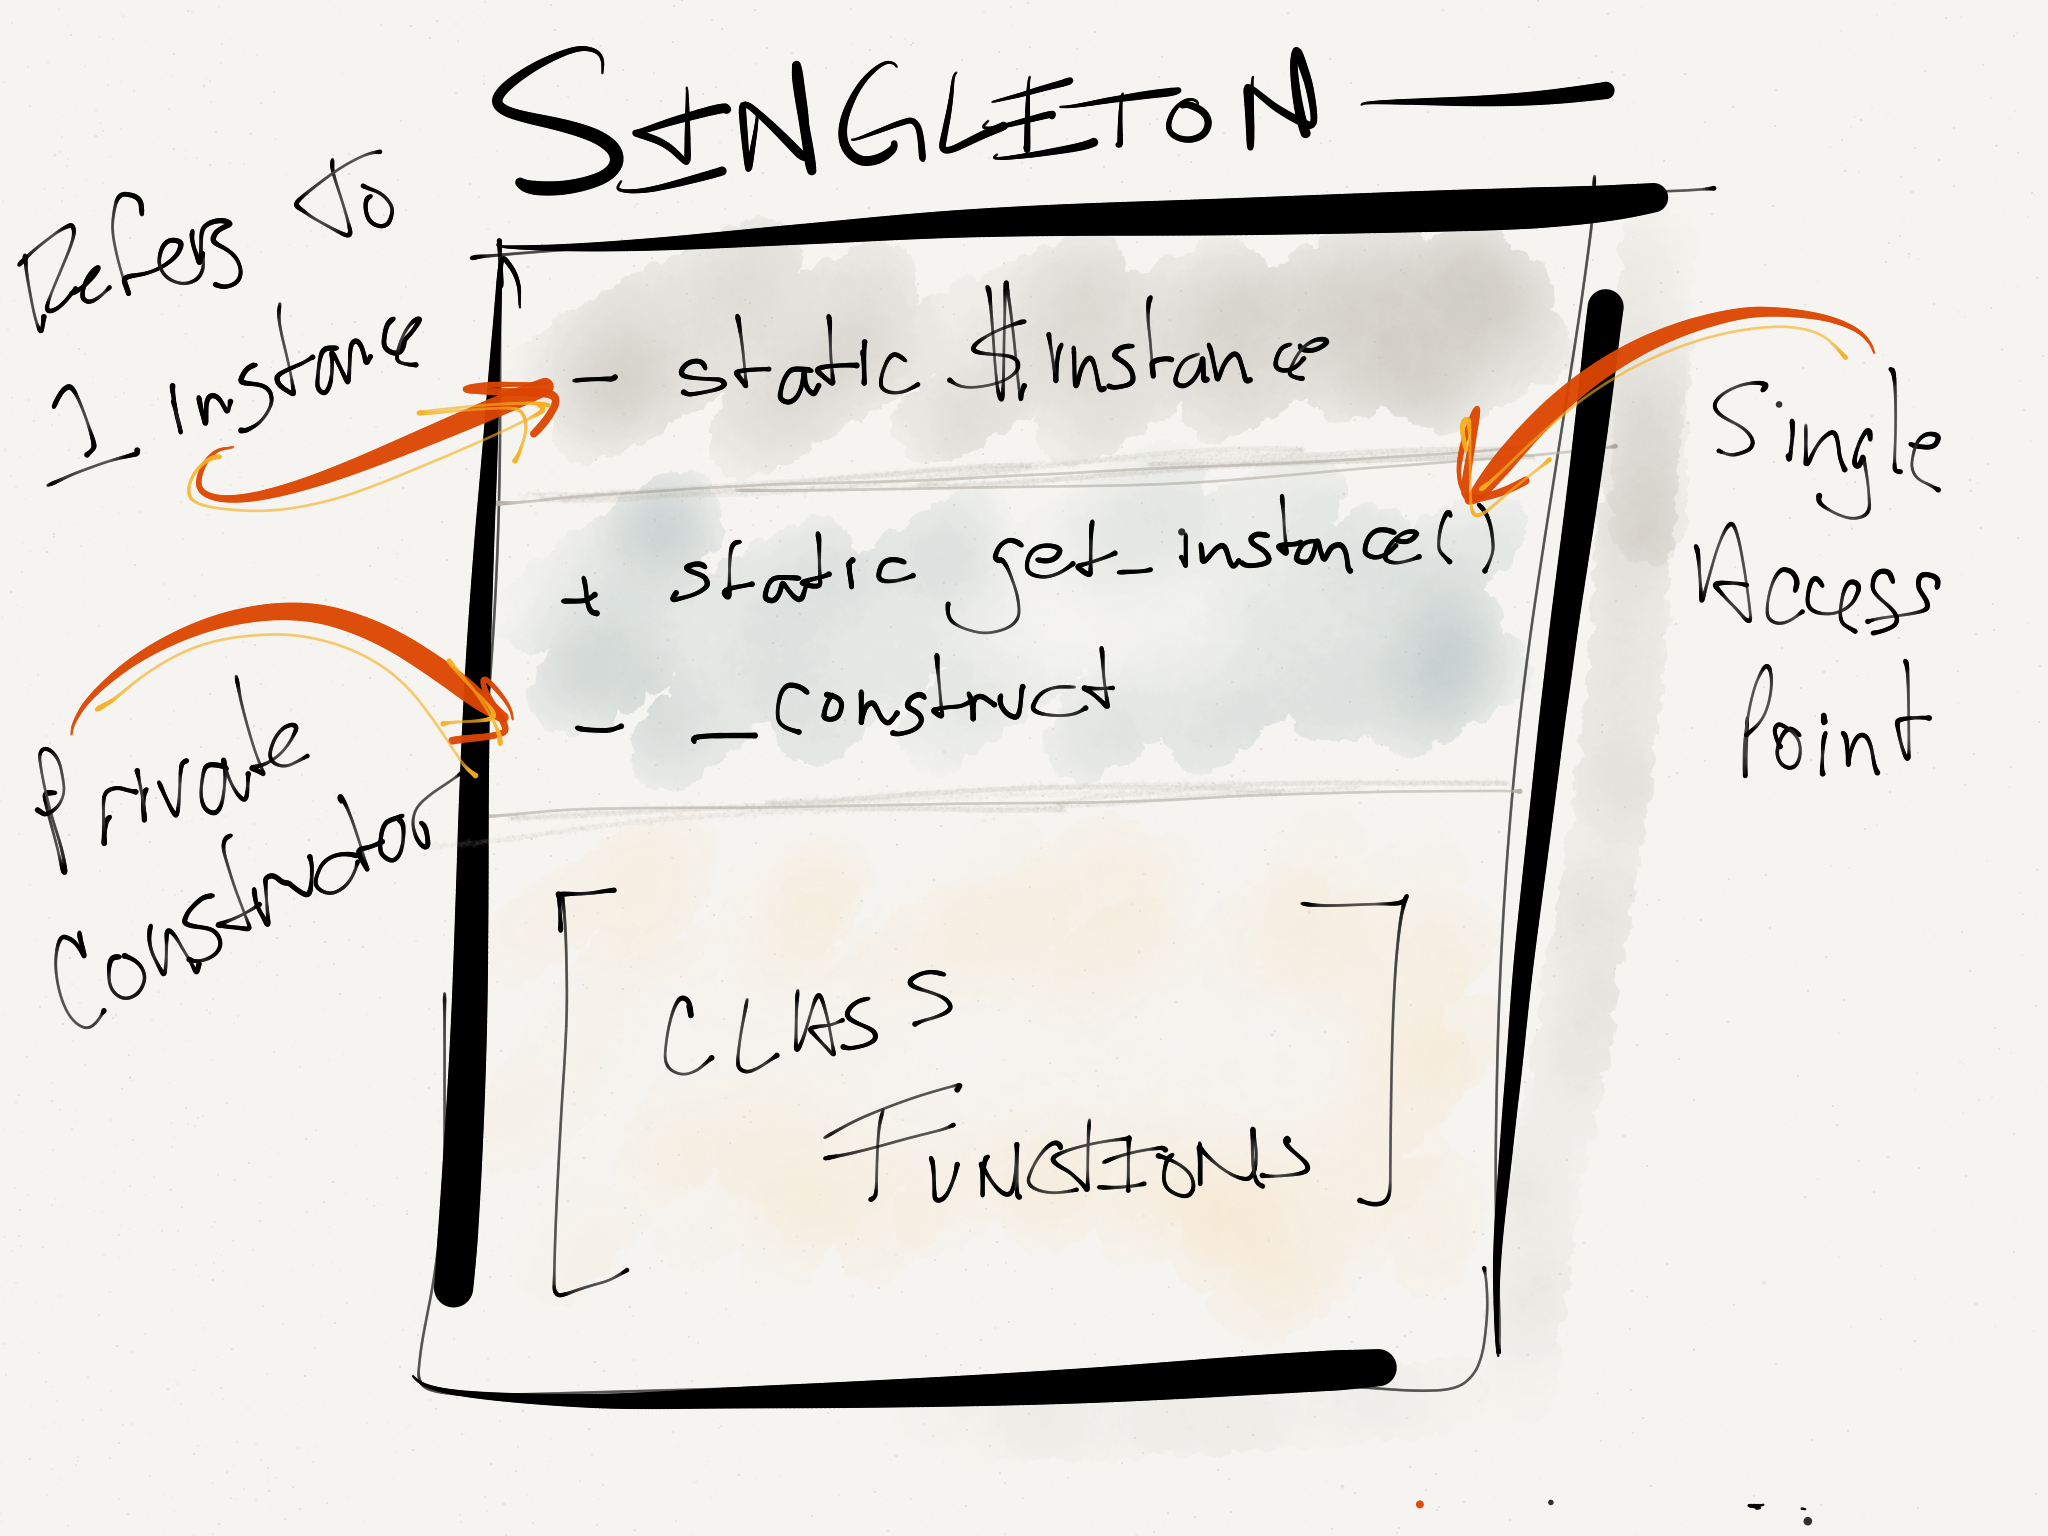
\includegraphics[width=1\textwidth]{images/singleton.png}
    \end{figure}
      \end{column}
       \hfill
      VS
      \begin{column}{.5\textwidth}
    \begin{figure}[train]
      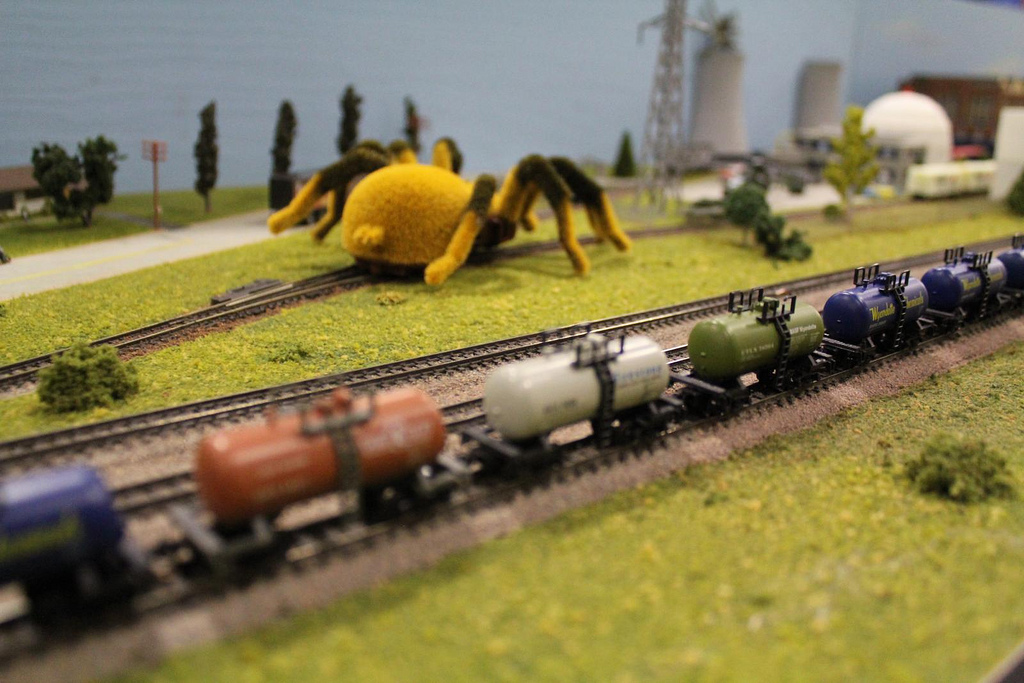
\includegraphics[width=1\textwidth]{images/demeter_train.jpg}
    \end{figure}
      \end{column}
    \end{columns}
\end{frame}

\begin{frame}{Law of Demeter}{Fluid interfaces}
\end{frame}

%=======================================================
\section{Running kuniri and output}
%=======================================================
\begin{frame}{Running}{Example}
  \begin{figure}[overview]
    
\includegraphics[width=0.6\textwidth]{images/terminal.png}
  \end{figure}
\end{frame}

%=======================================================
\section{Conclusions}
%=======================================================
\begin{frame}{Conclusion}{}
  \begin{itemize}
    \item A lot of work;
    \item Future works (improvements and new gems:
      \begin{enumerate}
        \item Improve state machine and ruby parser;
        \item Add new languages under kuniri;
        \item Shell tool;
        \item UML tool;
        \item Documentation tool;
        \item Simple metrics;
      \end{enumerate}
  \end{itemize}
\end{frame}

{\1
\begin{frame}[plain,noframenumbering]
  \finalpage{Thanks!}
\end{frame}}

\end{document}
